\section{Methodology}
%short introduction about CFD and the usage of ansys fluent
To understand the flow behaviour of various undertray geometry, fluid dynamics analysis is required. The rapid development of computational power has allowed more accurate and reliable results in computational analysis such as computational fluid dynamics (CFD)\cite{Andersson2011ComputationalEngineers}. The usage of CFD allows engineers to simplify the processes and achieve an accurate result in shorter time which allows engineers to do more iterations. 

\noindent The analysis is consist of 3 phase which are 2D enclosed \& open-flow, 3D bluff body, 3D undertray. The first phase is the 2D analysis which analyse the undertray variables on a Venturi-tube like geometry and open-flow analysis analyse a simple bluff body with similar undertray geometry. 3D bluff body will take the 2D geometry and extrude it as an 3D geometry which then analysed with the same undertray variables. Lastly is the 3D undertray where the optimised results from previous analysis will be used to determine the geometry of the final undertray design. To achieve realistic results, simplified traced body from the QFR 2021 car will be attached to the undertray. The process flow can be illustrated on figure \ref{fig:project methodology}. The work on this paper will be fully based on CFD which use ANSYS Fluent as a default working platform.

\begin{figure}[ht!]
    \centering
    \makebox[\textwidth]{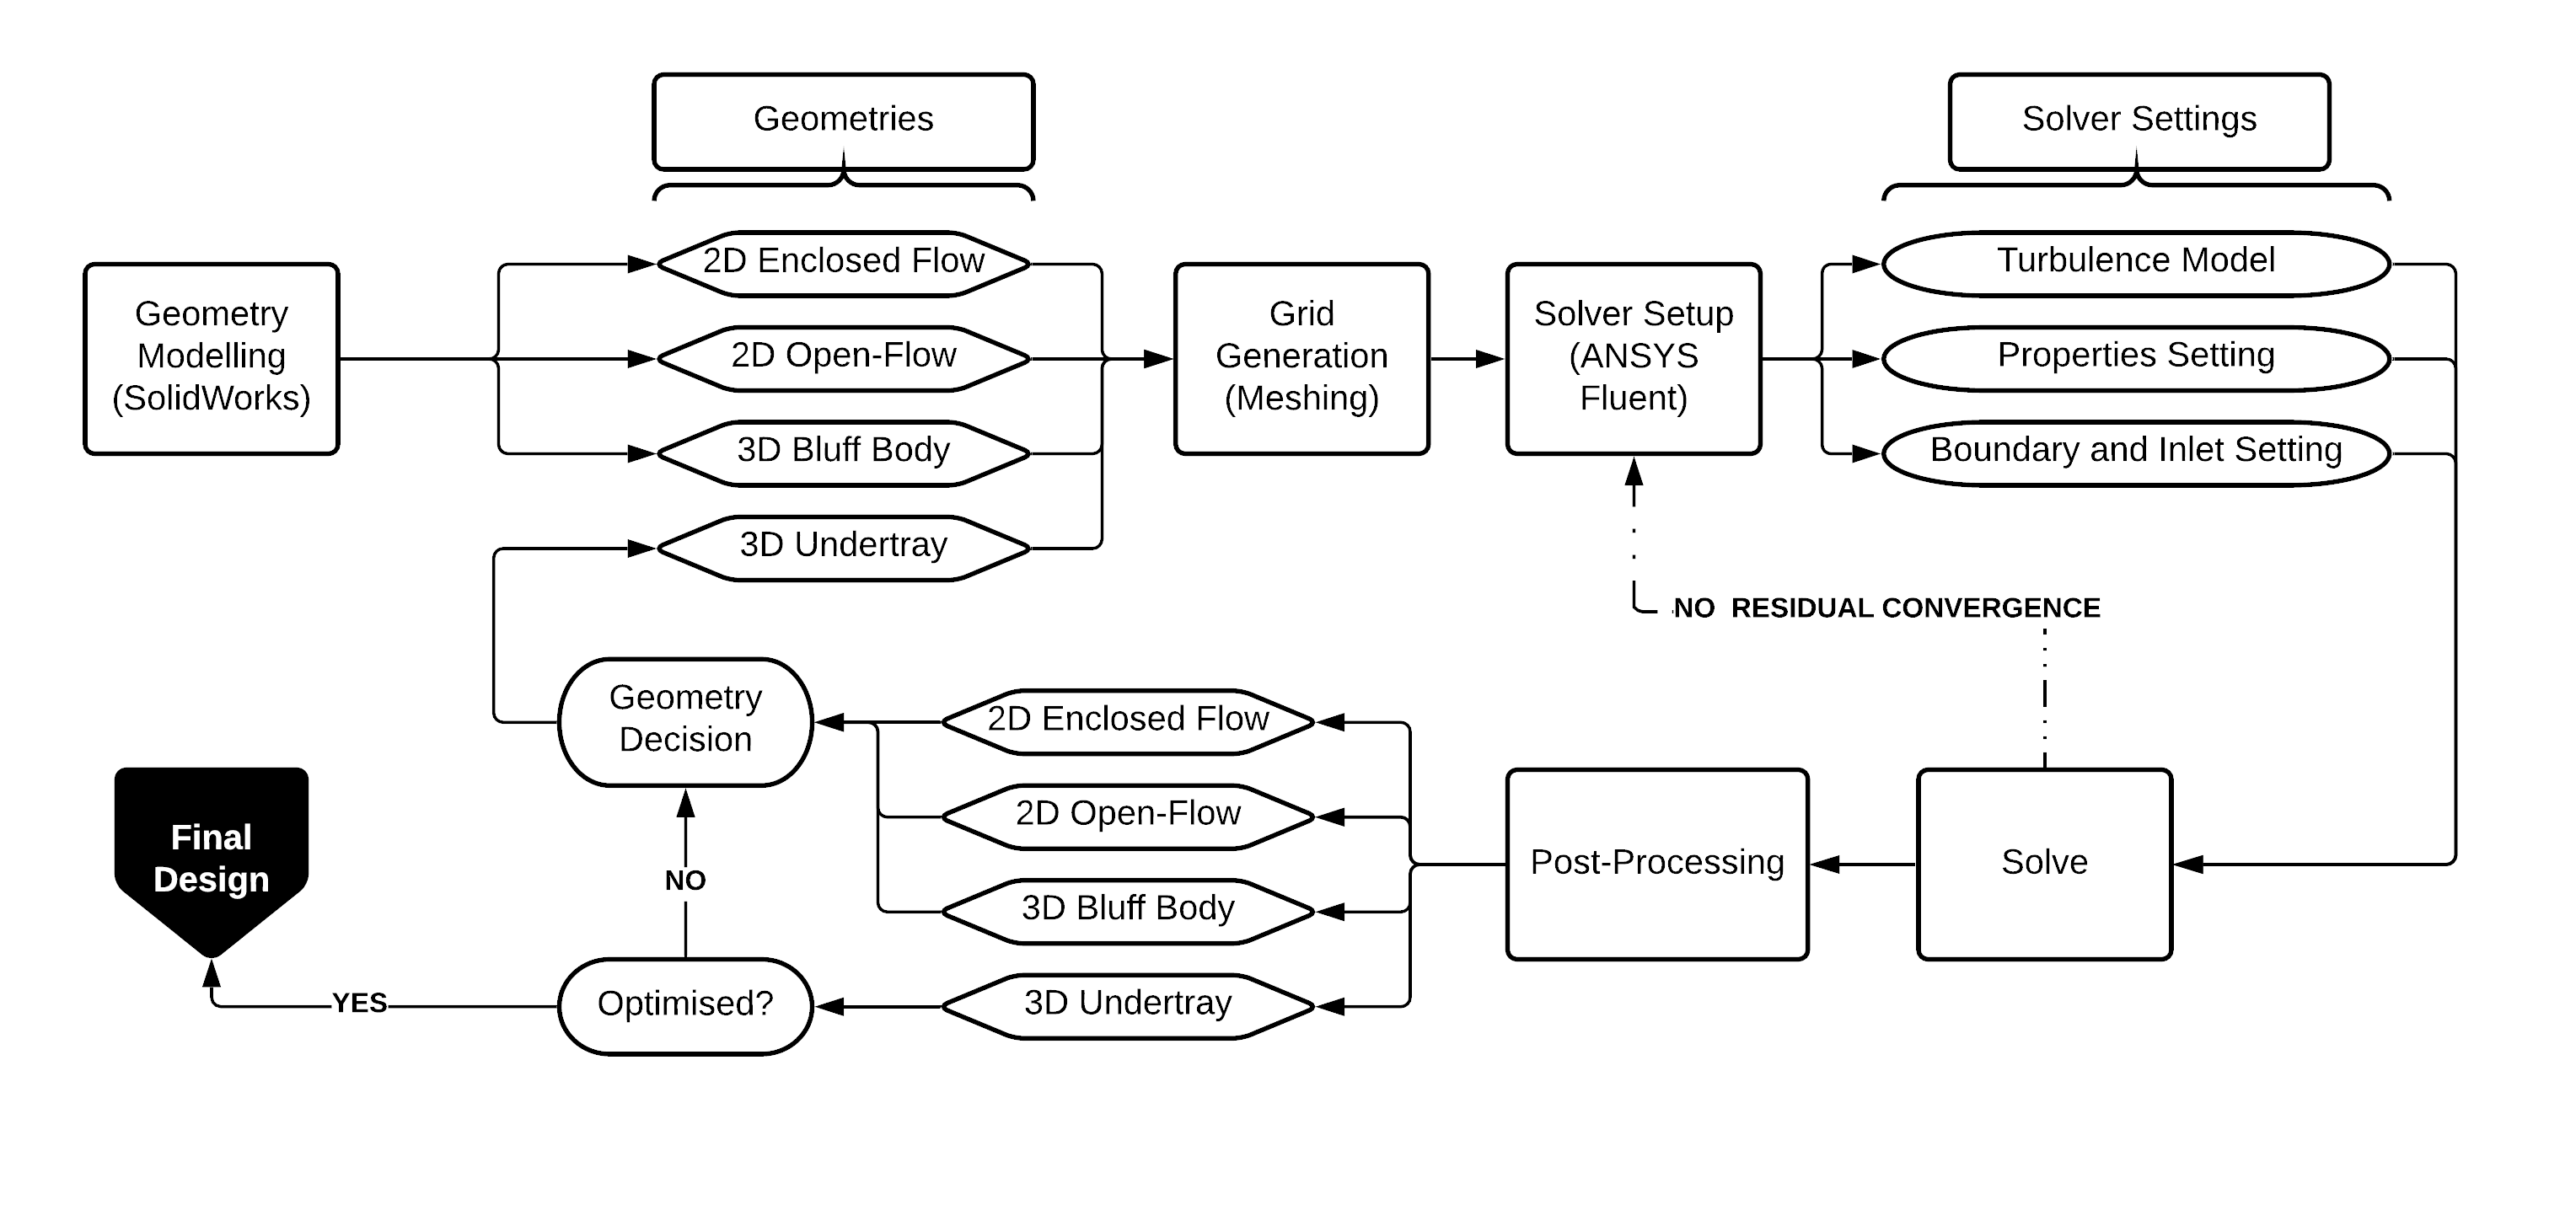
\includegraphics[scale=0.17]{Figures/project_methodology_chart.png}}
    \caption{Project Methodology Flow Chart}
    \label{fig:project methodology}
\end{figure}


\subsection{Pre-Processing}
\subsubsection{Geometry Generation}
Computer-aided geometry design (CAGD) is a modern systems in computational aided design to produce an external geometry\cite{Cummings2015AppliedAerodynamics}. The geometry changes of every analyses came in a step which results in high number of drawings, therefore, SolidWorks was used in this project to simplify the process. The SolidWorks geometry both 2D and 3D could be directly imported as active CAD which advantageous in saving time and memory.

\noindent In producing 2D geometry, SolidWorks are able to define the body and fluid surface at the same time which can be directly imported to mesh. The 3D bluff body can be directly imported to Design Modeller, however, there are number of step required since the SolidWorks geometry does not define the fluid body. To Create the fluid body, enclosure has to applied. Enclosure generates a geometry which surround the target body (bluff body) as a representation of the atmosphere. Then Boolean is applied to the fluid body, this process subtract the bluff body from the fluid body and create representation just for the flow around the bluff body which then  can be directly integrated to the meshing process on ANSYS Workbench.
%INSERT THE PHOTO OF 3D and 2D geometry

\subsubsection{Grid Generation (Meshing)}
The surface or body which have been defined becomes the basis for the meshing. Meshing app which integrated in ANSYS workbench provide a user-friendly, simple, and fast meshing generator. Due to the constrain of computational power and time, unstructured triangular (2D) and tetrahedral (3D) mesh were used. 

\noindent Looking back to the goal of the 2D and 3D bluff body simulation is to obtain and analyse the trend in geometry changes of an undertray, therefore, a non-detailed yet decent mesh could be generated. Local refinement around the body that affected by the fluid flow is recommended \cite{Lanfrit2005BestFLUENT} to achieve a reasonable results and flow representation especially around the undertray, moreover this technique allows larger mesh on the far field section less likely be affected or affecting the result. Other aspect of reasonable meshing is to be aware of the mesh properties such as skewness and growth ratio. For automotive application, it is recommended to have skewness less then 0.45 and maximum growth rate less than 20\% \cite{Lanfrit2005BestFLUENT}. 

\noindent One crucial facet of an undertray flow is generation of boundary layer and how it interacts with the moving floor, the accuracy of this aspect is depend on the quality of layer grid growth near the wall or wall function. To generate a good inflation layer, it is important to make sure the y+ value (first layer height grid) does not exceed the inner boundary layer region which can be done using the equation:

\begin{equation}
    y^+ = \frac{\rho U_\tau \partial y}{\mu}, where \quad U_\tau = \sqrt{\frac{\tau_w}{\rho}} = U \sqrt{\frac{1}{2}C_f}
\end{equation}

\noindent Figure \ref{fig:inflation layer} shows the illustration of y+ value on a wall function. The turbulence model on the solver also has to be a consideration in defining the y+ value, some turbulence modelling require a very low n y+ and some are able to tolerate high y+ value. Detail regarding y+ value in various turbulent model will be discussed on the next section. 

\begin{figure}[!ht]
    \centering
    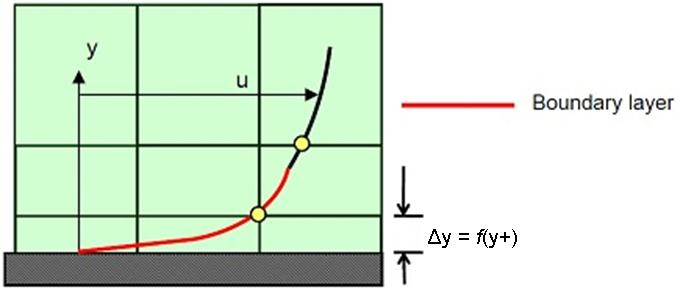
\includegraphics{Figures/inflation_layer.jpg}
    \caption{representation of y+ on a near wall function\cite{Inflate4Zealand}.}
    \label{fig:inflation layer}
\end{figure}



\subsection{Numerical Method}
%condition 
%turbulence modelling
-LEFT EMPTY-
LEAVE UNTIL 3D ANALYSIS IS DEFINED

\subsection{Post-Processing}
%very short talk about PST from ansys workbench
The final step is to analyse the flow characteristic and behaviour. PST is an app integrated in the ANSYS Workbench provide a fast and reliable platform to produce graphics such as contour, streamline, flow vector, etc which could be used to help analyse the overall aerodynamics of the body. 

